% !TEX root = ../main.tex
\section{Reasoning performance}
\label{sec:headlineresults}

We evaluate mathematical reasoning on GSM8K and MATH500, generating complete solutions through continuous latent denoising followed by a parallel token-decoding pass. Our comparisons address two questions: how strong a reasoning model this recipe produces, and how much inference is needed to obtain useful solutions. We report supervised and reward-fine-tuned models separately to distinguish the capabilities learned by the base recipe from the additional gains of post-training.

\paragraph{Evaluation setup.}
GSM8K contains 1,319 test problems, and MATH500 contains 500 problems drawn from MATH \citep{gsm8k,math,math500}. Our models use zero-shot prompts, a 1,024-token canvas, and async clocks $(2.5,2,1.5)$. GSM8K uses numerical-answer scoring; MATH500 uses Math-Verify \citep{mathverify}. The supervised endpoints are epoch 18 for ELF-B and epoch 21 for ELF-L; the NFT endpoints are updates 300, 500, and 600 for GSM8K ELF-B, GSM8K ELF-L, and MATH500 ELF-L, respectively. Supervised evaluations select ELF/prompt EMA $.9999/.9999$; NFT evaluations select $.99/.99$. Each headline accuracy averages eight sampling seeds at 64 denoising steps. The shared backbone runs once per denoising step and once for terminal decoding, giving 65 network function evaluations (NFEs); prompt encoding is performed once separately.

\subsection{Headline comparison}
\label{sec:headlinecomparison}
% !TEX root = ../main.tex
\begin{table}[t]
\caption{Mathematical reasoning, pass@1 (\%); our entries show mean $\pm$ sampling-seed standard deviation. Parameters are rounded to three significant digits. Embedding parameters include vocabulary input and output maps, counting tied weights once. In Other Params, $(+X)$ denotes additional parameters used once per response, including prompt encoding and terminal projection; frozen components are included. NFE counts diffusion denoising: $^{*}N$ denotes $N-1$ denoising calls for REPA+REG, whose reported budget includes a decoder call. Bold/underline mark first/second place within each of the two sub-billion continuous-backbone groups.}
\label{tab:headlinecomparison}
\centering\small
\setlength{\tabcolsep}{2pt}
\begin{tabular}{@{}lrrrrr@{}}
\toprule
Model & \shortstack{Embedding\\Params (M)} & \shortstack{Other\\Params (M)} & NFE & GSM8K & MATH500\\
\midrule
\multicolumn{6}{@{}l}{\textit{Autoregressive}}\\
Qwen3-0.6B-Base \citep{qwen3} & 156 & 440 & --- & 59.59 & ---\\
Qwen3-0.6B, thinking \citep{qwen3} & 156 & 440 & --- & --- & 77.60\\
\midrule
\multicolumn{6}{@{}l}{\textit{Discrete diffusion / blockwise diffusion}}\\
LLaDA-8B-Base \citep{llada} & 1,040 & 6,980 & 1,024 & 70.30 & ---\\
Dream-v0-Base-7B \citep{dream} & 1,090 & 6,530 & 256 & 77.20 & ---\\
SDAR-1.7B-Chat \citep{sdar} & 622 & 1,410 & 4/block & 80.10 & 63.20\\
\midrule
\multicolumn{6}{@{}l}{\textit{Continuous diffusion / flow: denoising backbone below 200M}}\\
$\mathbb S$-FLM \citep{hyperspherical} & 75.5 & 87.5 & 1,024 & 18.00$^\dagger$ & ---\\
FMLM+ Init \citep{posterior} & 75.5 & 92 & 64 & 33.60$^\dagger$ & ---\\
REPA+REG-B \citep{scalingdlm} & 311 & 104 $(+441)$ & $^{*}64$ & 38.11 & ---\\
\textbf{ELF-B, pre-NFT (ours)} & 545 & 90.4 $(+45.8)$ & 64 & \accsd{\underline{39.17}}{0.63} & ---\\
\textbf{ELF-B, post-NFT (ours)} & 545 & 90.4 $(+45.8)$ & 64 & \accsd{\textbf{42.16}}{0.88} & ---\\
\midrule
\multicolumn{6}{@{}l}{\textit{Continuous diffusion / flow: denoising backbone 200M--1B}}\\
REPA+REG-L \citep{scalingdlm} & 311 & 652 $(+442)$ & $^{*}64$ / $^{*}128$ & 55.96 & 13.39\\
\textbf{ELF-L, pre-NFT (ours)} & 545 & 638 $(+123)$ & 64 & \accsd{\underline{58.67}}{0.69} & \accsd{\underline{21.18}}{0.70}\\
\textbf{ELF-L, post-NFT (ours)} & 545 & 638 $(+123)$ & 64 & \accsd{\textbf{63.74}}{0.83} & \accsd{\textbf{24.68}}{1.27}\\
\midrule
\multicolumn{6}{@{}l}{\textit{Continuous diffusion / flow: larger backbones (reference)}}\\
MLFM \citep{mlfm} & 123 & 1,220 & 256 & 31.24 & ---\\
TESS 2, GSM8K FT \citep{tess2} & 262 & 6,740 & 1,000 & 68.9$^\ddagger$ & ---\\
\bottomrule
\end{tabular}
\vspace{3pt}
\parbox{\linewidth}{\footnotesize Our rows use eight seeds, async $(2.5,2,1.5)$, SCCFG 2 for GSM8K, and SCCFG 3 for MATH500; the standard-deviation definition and full summaries appear in Appendix~\ref{app:seedvariability}. External accuracies and sampling budgets follow the authors' reports; $^\dagger$Python scoring, $^\ddagger$figure-derived accuracy. GSM8K uses 4-shot Qwen/LLaDA, 8-shot Dream/TESS~2, and zero-shot prompts for ours. SDAR uses four steps per four-token block. A slash separates GSM8K/MATH500 budgets. REPA+REG includes its frozen Qwen prompt encoder and the authors' rounded REPA-projector counts. MLFM includes unmerged adapters; SDAR counts both untied vocabulary maps. Our vocabulary maps are called once. NFE excludes prompt encoding and terminal decoding.}
\end{table}


Table~\ref{tab:headlinecomparison} separates autoregressive, discrete-diffusion, and continuous-diffusion models. We use the comparison papers' reported accuracies, retaining their evaluation settings. The parameter columns distinguish vocabulary-sized maps from the remaining network weights, including frozen components. This is particularly relevant for our inherited Qwen vocabulary: its input and output maps contain 544.69M parameters, while the denoising backbones contain 90.44M and 638.15M parameters for ELF-B and ELF-L. The learned prompt encoder and terminal decoder add computation once per response; neither model executes the Qwen teacher Transformer during generation.

Strong performance is already present before reward-based post-training. Supervised ELF-B achieves 39.17\% on GSM8K, exceeding FMLM+ Init's 33.60\%, while supervised ELF-L reaches 58.67\%. On MATH500, supervised ELF-L reaches 21.18\%, compared with 13.39\% for the concurrent REPA+REG-L model at 128 NFEs \citep{posterior,scalingdlm}. NFT further raises ELF-L to 63.74\% on GSM8K and 24.68\% on MATH500. These results strengthen the evidence that relatively compact continuous denoisers can support multi-step reasoning, with the larger autoregressive and discrete models providing context for the remaining performance gap.

The headline MATH500 rows use SCCFG 3, the stronger pass@1 setting in our follow-up guidance sweep. At the same checkpoints, SCCFG 2 gives 18.85\% before NFT and 23.60\% afterward. We retain SCCFG 2 throughout the inference-allocation figures below so that all displayed curves share the original common guidance setting.

\subsection{Reasoning at lower NFE}
\label{sec:headlinelownfe}
% !TEX root = ../main.tex
\begin{table}[t]
\caption{Reasoning at lower denoising NFE, pass@1 (\%); our entries show mean $\pm$ sampling-seed standard deviation. Bold/underline indicate first/second place within each benchmark and backbone-scale block. A leading $^{*}$ marks a result with one fewer denoising call than the column heading: REPA+REG includes terminal decoding in its reported NFE. FMLM+ values are from its Table~8; REPA+REG values are from its Tables~11 and~15 and use early stopping \citep{posterior,scalingdlm}.}
\label{tab:headlinelownfe}
\centering\small
\setlength{\tabcolsep}{7pt}
\begin{tabular}{@{}lrrrr@{}}
\toprule
Method & 8 NFE & 16 NFE & 32 NFE & 64 NFE\\
\midrule
\multicolumn{5}{@{}l}{\textit{GSM8K: approximately 100M denoising backbone}}\\
FMLM+ Init & 15.10 & 26.10 & 31.80 & 33.60\\
REPA+REG-B & $^{*}$26.20 & $^{*}$34.42 & $^{*}$37.15 & $^{*}$38.11\\
ELF-B, pre-NFT (ours) & \accsd{\underline{26.40}}{0.87} & \accsd{\underline{34.48}}{0.94} & \accsd{\underline{37.80}}{1.20} & \accsd{\underline{39.17}}{0.63}\\
ELF-B, post-NFT (ours) & \accsd{\textbf{30.08}}{0.87} & \accsd{\textbf{37.77}}{0.84} & \accsd{\textbf{41.13}}{0.94} & \accsd{\textbf{42.16}}{0.88}\\
\midrule
\multicolumn{5}{@{}l}{\textit{GSM8K: approximately 650M denoising backbone}}\\
REPA+REG-L & $^{*}$47.34 & $^{*}$52.89 & $^{*}$55.04 & $^{*}$55.96\\
ELF-L, pre-NFT (ours) & \accsd{\underline{49.41}}{0.86} & \accsd{\underline{55.33}}{0.91} & \accsd{\underline{57.88}}{1.03} & \accsd{\underline{58.67}}{0.69}\\
ELF-L, post-NFT (ours) & \accsd{\textbf{54.84}}{0.92} & \accsd{\textbf{60.55}}{0.69} & \accsd{\textbf{62.47}}{0.82} & \accsd{\textbf{63.74}}{0.83}\\
\midrule
\multicolumn{5}{@{}l}{\textit{MATH500: approximately 650M denoising backbone}}\\
REPA+REG-L & $^{*}$9.76 & $^{*}$11.53 & $^{*}$12.40 & $^{*}$13.31\\
ELF-L, pre-NFT (ours) & \accsd{\underline{15.23}}{1.16} & \accsd{\underline{17.93}}{1.30} & \accsd{\underline{19.65}}{1.37} & \accsd{\underline{21.18}}{0.70}\\
ELF-L, post-NFT (ours) & \accsd{\textbf{17.45}}{1.33} & \accsd{\textbf{20.93}}{1.26} & \accsd{\textbf{22.60}}{1.58} & \accsd{\textbf{24.68}}{1.27}\\
\bottomrule
\end{tabular}
\vspace{3pt}
\parbox{\linewidth}{\footnotesize Our checkpoints are fixed across columns, using SCCFG 2 for GSM8K and SCCFG 3 for MATH500. Means use 64, 32, 16, and 8 sampling seeds from left to right; Appendix~\ref{app:seedvariability} gives the standard-deviation definition and full summaries. FMLM+ grades Python solutions; REPA+REG and our models produce natural-language reasoning.}
\end{table}


The gains persist when inference is shortened. At 17 NFEs, supervised ELF-B reaches 34.48\% on GSM8K, exceeding FMLM+ Init's 33.60\% at 64 NFEs. At only nine NFEs, supervised ELF-L reaches 49.41\% on GSM8K and 15.23\% on MATH500; the latter exceeds REPA+REG-L's 13.39\% at 128 NFEs. NFT improves accuracy at every evaluated depth in Table~\ref{tab:headlinelownfe}. Thus useful reasoning emerges well before our longest denoising trajectory, without training a separate few-step student. These are comparisons of reported operating points; differences in training data, prompting, and model architecture remain, and NFE does not equate FLOPs across methods.

\subsection{Refining an answer or drawing more answers}
\label{sec:headlinebudget}
An additional opportunity comes from allocating inference across independent solutions. For $k$ samples with $S$ denoising steps each, we use $kS$ as an interpretable budget. Oracle pass@$k$ measures whether at least one sample is correct. Majority voting instead selects the most frequent final answer after grouping equivalent answers, without consulting the reference. We average over tied winners and sample subsets using the same saved generations. The four denoising depths $S\in\{8,16,32,64\}$ have $64,32,16,8$ draws per problem, respectively, so each reaches a total budget of 512 steps.

\begin{figure}[t]
\centering
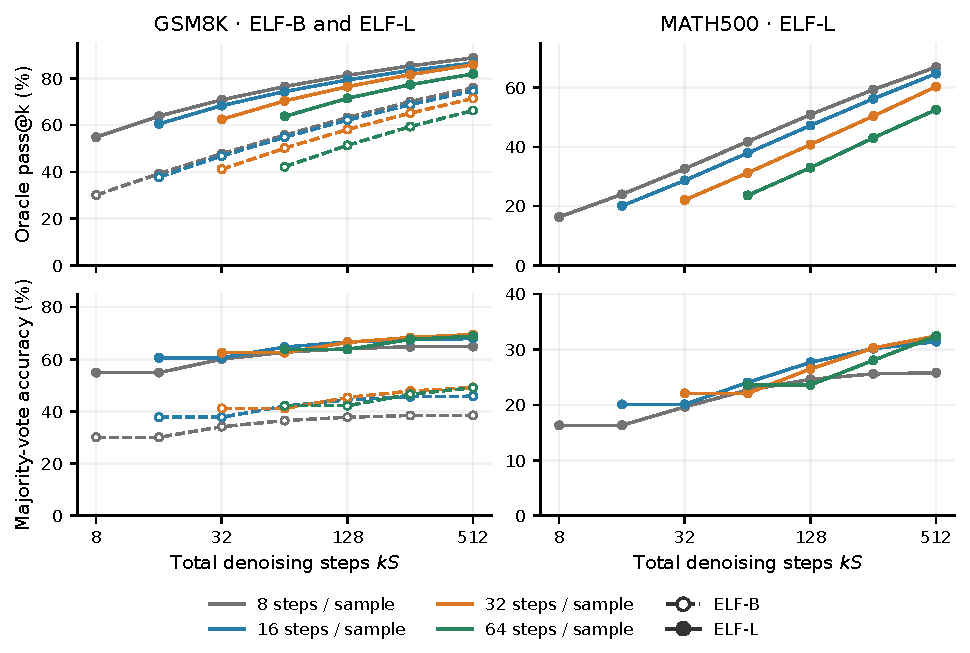
\includegraphics[width=\linewidth]{figures/headline_nft_budget_compact.pdf}
\caption{Post-NFT reasoning across inference allocations, with SCCFG 2 throughout. Colors identify denoising steps per sample. GSM8K ELF-B uses hollow circles and dashed lines; ELF-L uses filled circles and solid lines. Upper panels show oracle pass@$k$; lower panels show majority-vote accuracy. Each curve reaches 512 total denoising steps. Points average over the complete sample cohort at each depth; lines connect evaluated allocations. The horizontal axis counts denoising steps, while total backbone calls are $k(S+1)$, with prompt encoding additional.}
\label{fig:headlinenftbudget}
\end{figure}

Figure~\ref{fig:headlinenftbudget} shows two distinct uses of additional samples. Short trajectories provide broader oracle coverage at a fixed total step budget, while longer trajectories more reliably concentrate samples on a correct answer. On MATH500 after NFT, 64 samples with eight steps each reach 67.00\% oracle accuracy, compared with 52.60\% for eight samples with 64 steps each. Voting reverses this preference: the corresponding accuracies are 25.79\% and 32.42\%. The comparison therefore exposes a meaningful choice between exploring more candidate solutions and making the returned answer more reliable.

\begin{figure}[t]
\centering
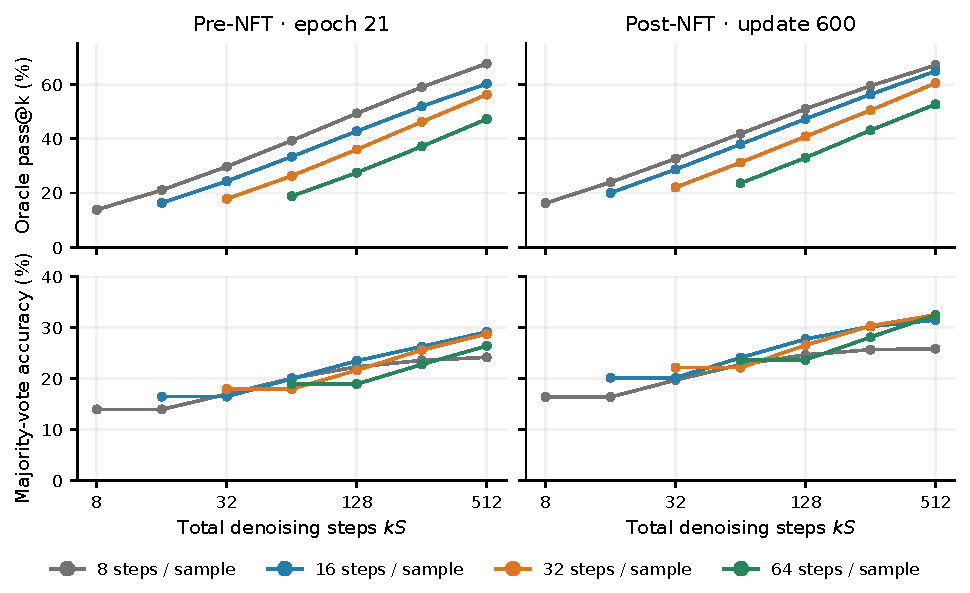
\includegraphics[width=\linewidth]{figures/headline_math_stages_sccfg2.pdf}
\caption{MATH500 inference allocation before and after NFT, holding SCCFG at 2. The supervised model already benefits from drawing multiple solutions; NFT improves both single-sample accuracy and the accuracy obtained by voting. Colors and sample budgets match Figure~\ref{fig:headlinenftbudget}. SCCFG 3 further improves pass@1, as reported in Tables~\ref{tab:headlinecomparison} and~\ref{tab:headlinelownfe}; its effect on higher-$k$ oracle coverage is not uniformly positive.}
\label{fig:headlinemathstages}
\end{figure}

Figure~\ref{fig:headlinemathstages} places this tradeoff alongside the supervised model. The preference for many short trajectories under oracle selection, and for longer trajectories under majority voting, is visible in both training stages. This distinction is useful when choosing how the model will be deployed: oracle coverage measures the potential available to a downstream selector, while majority voting measures an answer-selection procedure that can be used directly.

\subsection{Generated solutions}
% !TEX root = ../main.tex
\begin{figure}[p]
\centering
\setlength{\fboxsep}{8pt}
\fbox{\begin{minipage}{0.94\linewidth}
\small
\textbf{GSM8K: reasoning across successive changes}\par\medskip
\textbf{Problem.} A new program had 60 downloads in the first month. The number of downloads in the second month was three times as many as the downloads in the first month, but then reduced by 30% in the third month. How many downloads did the program have total over the three months?

\medskip\textbf{Generated solution.}\par\smallskip
Let's break down the downloads for the program month by month.

In the first month, the program had 60 downloads.

In the second month, the program had three times as many as the downloads in the first month, so it had 60 * 3 = 180 downloads.

In the third month, the downloads were reduced by 30%, which means it had 180 - (180 * 30 / 100) = 180 - 54 = 126 downloads.

To find the total number of downloads over the three months, we add up the downloads from each month: 60 + 180 + 126 = 240 + 126 = 366

Thus, the program had a total of $\boxed{366}$ downloads over the three months.
\end{minipage}}

\medskip
\fbox{\begin{minipage}{0.94\linewidth}
\small
\setlength{\abovedisplayskip}{4pt}
\setlength{\belowdisplayskip}{4pt}
\textbf{MATH500: evaluating a rational function}\par\medskip
\textbf{Problem.} If $f(x) = \frac{3x-2}{x-2}$, what is the value of $f(-2) +f(-1)+f(0)$? Express your answer as a common fraction.

\medskip\textbf{Generated solution.}\par\smallskip
To find the value of $f(-2)+f(-1)+f(0)$ we need to substitute $x=-2, x=-1,$ and $x=0$ into the function $f(x)$.

For $f(-2)$:
\[ f(-2) = \frac{3(-2) - 2}{-2 - 2} = \frac{-6 - 2}{-4} = \frac{-8}{-4} = 2 \]

For $f(-1)$:
\[ f(-1) = \frac{3(-1) - 2}{-1 - 2} = \frac{-3 - 2}{-3} = \frac{-5}{-3} = \frac{5}{3} \]

For $f(0)$:
\[ f(0) = \frac{3(0) - 2}{0 - 2} = \frac{-2}{-2} = 1 \]

Now we can add these together to find the sum:
\[ f(-2) + f(-1) + f(0) = 2 + \frac{5}{3} + 1 = \frac{11}{3} + 1 = \frac{11}{3} + \frac{3}{3} = \frac{14}{3} \]

\[ \boxed{\frac{14}{3}} \]
\end{minipage}}
\caption{Correct generations from ELF-L at 64 denoising steps (65 NFEs), async $(2.5,2,1.5)$, SCCFG 2, and seed 42. GSM8K uses NFT update 500; MATH500 uses NFT update 600. Model text is unchanged, with mathematical markup typeset for readability. Both answers and the intermediate calculations are correct.}
\label{fig:headlineexamples}
\end{figure}

Figure~\ref{fig:headlineexamples} presents one correct GSM8K generation and one correct MATH500 generation from the post-NFT ELF-L models. The solutions combine intermediate calculations into a final answer: successive multiplicative changes in the GSM8K example, and substitution followed by rational arithmetic in the MATH500 example. Both are drawn from saved benchmark generations and retain the original model text.
